\documentclass[compress]{beamer}
\usepackage{beamerthemeproyxetex}


%\useoutertheme[footline=authorinstitutetitle]{miniframes}
%\usecolortheme{whale}
%\usecolortheme{orchid}
%\useinnertheme{rounded}


\title{FoLiA: Format for Linguistic Annotation}
\author{Maarten van Gompel}
\date{24-03-2011}
\usepackage{graphicx}
\usepackage{listings}
\usepackage{color}
\lstset{% general command to set parameter(s)
basicstyle=\footnotesize,
keywordstyle=\color{black}\bfseries\underbar,
identifierstyle=\color{black}\bfseries\underbar,
stringstyle=\ttfamily,
}


\begin{document}

\begin{frame}
	\titlepage\smallraccoon\ilkuvt
\end{frame}

\section{Introduction}

\begin{frame}{Introduction}

    \begin{block}{Annotation formats in the field}
        \begin{itemize}
            \item Many ad-hoc and old-style annotation formats (CGN, Tadpole column format) 
            \item Many theoretic and specialised annotation formats with limited scope
            \item OVerly rich document encoding formats (TEI)
            \item Many conversions needed
            \item De-facto-standard for various ILK projects: SoNaR/DCOI
        \end{itemize}
    \end{block}

\end{frame}
    
\begin{frame}

    \begin{block}{Limits Tadpole/Frog columned format}
        \begin{itemize}
            \item Simplistic format, lacking expressiveness of XML
            \item Six/seven columns currently, covering full screen width
            \item Lacking even expressiveness to fully output Frog's data!
        \end{itemize}
    \end{block}
    
\end{frame}
    
    
\begin{frame}
    \begin{block}{Limits of DCOI}
        \begin{itemize}
            \item Not expressive enough for many kinds of annotation (such as sense annotation, correction annotation)
            \item Can't encode annotators
            \item Can't encode alternatives
        \end{itemize}
    \end{block}
    
\end{frame}    



\begin{frame}{Objectives}
    \begin{block}{Objectives (1/2)}
        \textbf{Objectives: Expressability, Extensability, Uniformity}
        \begin{itemize}        
            \item One generalised rich common XML-based format, supporting almost all we do at ILK
            \item Uniform and consistent paradigm for annotations of various kinds
            \item Built from a bottom-up application-oriented perspective            
            \item Not committing to any particular tagset or language            
            \item Encoding many different annotation aspects similtaneously in a single XML file
            \item Support for sense annotation (DutchSemCor)
        \end{itemize}        
    \end{block}
\end{frame}
            

\begin{frame}{Objectives}
    \begin{block}{Objectives (2/2)}
        \textbf{Objectives: Expressability, Extensability, Uniformity}
        \begin{itemize}                    
            \item Support for complex corrections (Valkuil $+$ Ticcl)
            \item Support for NER (HITIME)
            \item Support in Frog for reading and writing this format            
            \item Founded on the DCOI format (our de-facto standard)
            \item Inter-operability with ISO Data Category Registry
            \item Unicode compliant
            \item Fully open-source
        \end{itemize}        
    \end{block}
\end{frame}

\begin{frame}{Annotations}
    \begin{block}{Supported Annotations (1/2)}
        FoLiA supports the following linguistic annotations:
        \begin{itemize}
            \item Part-of-Speech tags (with features)
            \item Lemmatisation
            \item Spelling corrections on both a tokenised as well as an untokenised level.
            \item Domain tagging
            \item Semantic sense annotation (to be used in DutchSemCor)
        \end{itemize}
        

    \end{block}
\end{frame}
            
\begin{frame}{Annotations}
    \begin{block}{Supported Annotations (2/2)}
        FoLiA supports the following linguistic annotations:
        \begin{itemize}            
            \item Named Entities / Multi-word units
            \item Syntactic Parses
            \item Dependency Relations
            \item Chunking
            \item Corrections
        \end{itemize}
    
        More to be added when needed (in collaboration with partners)

    \end{block}
\end{frame}

\section{Format}

\begin{frame}[fragile]
\frametitle{Format: Overall skeleton}
\begin{lstlisting}[language=xml]
<?xml version="1.0" encoding="utf-8"?>
<FoLiA xmlns="http://ilk.uvt.nl/FoLiA"
  xmlns:xsi="http://www.w3.org/2001/XMLSchema-instance"
  xml:id="example">
  <metadata>    
    <annotations>
      ...
    </annotations>    
    <!-- (Here IMDI or CMDI metadata can be inserted) -->
  </metadata>
  <text xml:id="example.text">
     ...
  </text>
</FoLiA>  
\end{lstlisting}
\end{frame}

\begin{frame}
    \begin{block}{Characteristic of overall format}
      \begin{enumerate}
        \item Unique identifier for document as a whole
        \item Metadata 
        \begin{itemize}
            \item Annotations - Declaration of all used annotations
            \item May hold IMDI or CMDI metadata
        \end{itemize}
        \item Text        
      \end{enumerate}
    \end{block}
\end{frame}



\begin{frame}[fragile]
\frametitle{Format: Basic structure}
\begin{lstlisting}[language=xml]
<p xml:id="TEST.p.1">
    <t>This is a test. It has two sentences.</t>
    <s xml:id="TEST.p.1.s.1">        
        <t>This is a test.</t>
        <w xml:id="TEST.p.1.s.1.w.1"><t>This</t></w>
        <w xml:id="TEST.p.1.s.1.w.2"><t>is</t></w>
        ..
    </s><s xml:id="TEST.p.1.s.2">...</s>                
</p>                
\end{lstlisting}
    
\end{frame}

\begin{frame}
    \begin{block}{Characteristics of basic structure}
      \begin{enumerate}
        \item \textbf{Structure Elements}: Paragraphs, Sentences, Words/Tokens  
        \item More: Division, Head, List, ListItem, Figure, Gap...
        \item Unique identifiers (DCOI style by convention)
        \item Text element (t) holds actual text. May occur untokenised on higher levels as well.
      \end{enumerate}
    \end{block}
\end{frame}
        
        

\section{Paradigm}

\begin{frame}
    \begin{block}{Paradigm: Annotation Categories}
            
        
        Three categories of annotation:    
        \begin{itemize}            
            \item \textbf{Structure Annotation} - Elements denoting document structure
            \begin{itemize}
                \item {\footnotesize E.g: Divisions, Header, Paragraphs, Sentences, Lists, Figures, Gaps }
            \end{itemize}
            \item \textbf{Token Annotation} - Linguistic Annotations pertaining to a single token (inline annotation)
            \begin{itemize}
                \item {\footnotesize E.g: Part of Speech Annotation, Lemma Annotation, Lexical Semantic Sense Annotation }
            \end{itemize}
            \item \textbf{Span Annotation} - Linguistic Annotations spanning over multiple tokens (standoff annotation)
            \begin{itemize}
                \item {\footnotesize E.g: Syntactic Parses, Dependency Relation, Entities/Multi-word Units}
            \end{itemize}
        \end{itemize}
            
    \end{block}
\end{frame}

        
\begin{frame}
    \begin{block}{Paradigm: Common Attributes}
            
        FoLiA Attributes common to the paradigm.
        \begin{itemize}
            \item \textbf{ID} - A unique ID for the element
            \item \textbf{Set} - Identifier of a particular (tag)set
            \item \textbf{Class} - One class from the specified set
            \item \textbf{Annotator} - An open identifier for the user/system who provided the annotation
            \item \textbf{Annotator type} - ``auto'' or ''manual''
            \item \textbf{Confidence} - A confidence value between one and zero.
            \item \textbf{N} - A sequential number (for numbered divisions/sections, list items, etc)            
        \end{itemize}
            
    \end{block}
\end{frame}


\begin{frame}
        \frametitle{Paradigm: Schematic}
        \begin{center}
        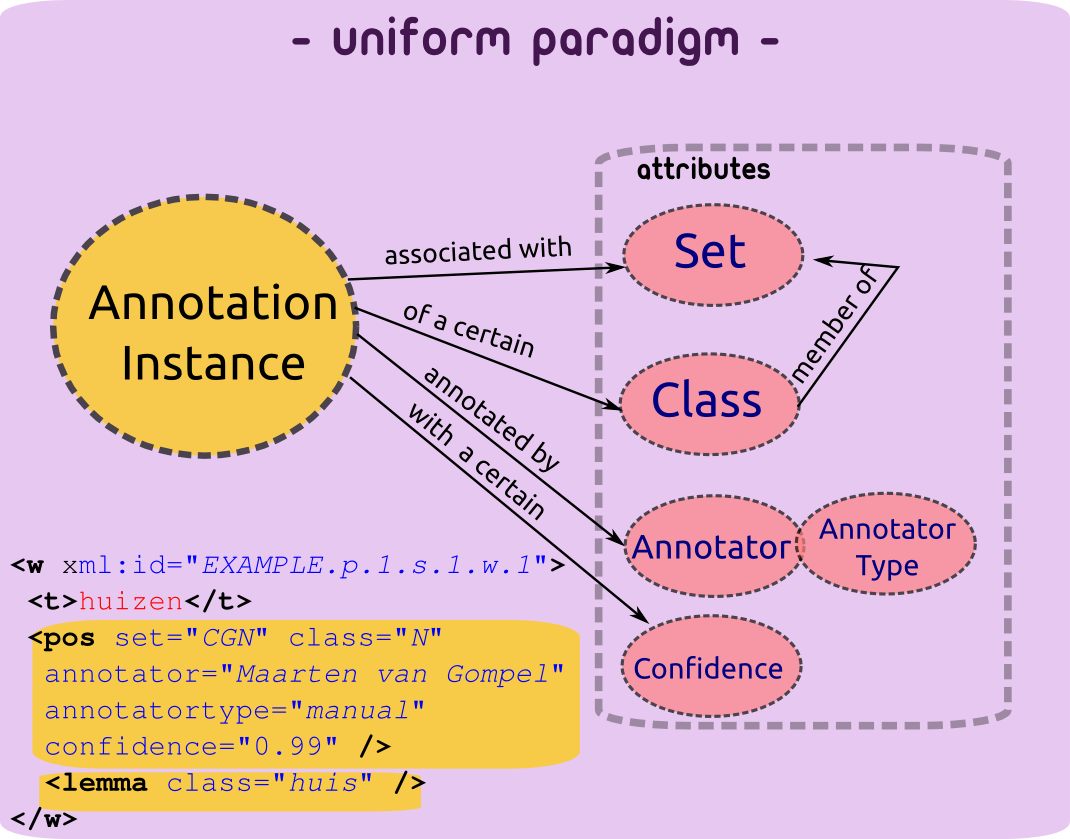
\includegraphics[width=90.0mm]{paradigm.png}
        \end{center}
\end{frame}


\section{Token Annotation}

\begin{frame}[fragile]
    \begin{block}{Token Annotation}
        Token annotation occurs within the scope of a word/token (\emph{w}) element.
    \end{block}
    \begin{example}
       PoS and Lemma Annotation:
\begin{lstlisting}[language=xml]
<w xml:id="example.p.1.s.1.w.2">
    <t>boot</t>
    <pos set="brown" class="n" 
     annotator="Maarten van Gompel" annotatortype="manual" />
    <lemma set="english-lemmas" class="boot" />
</w>                         
\end{lstlisting}        
    \end{example}
\end{frame}


\begin{frame}[fragile]
    \begin{block}{Token Annotation}
        All annotations need to be declared in the metadata:
        \begin{itemize}
            \item Default sets and annotator \emph{may} be predefined at this level
        \end{itemize}
    \end{block}
    \begin{example}
\begin{lstlisting}[language=xml]
<metadata>
 <annotations>
  <token-annotation />
  <pos-annotation set="brown" annotator="Maarten van Gompel"
    annotatortype="manual"/>
  <lemma-annotation />
 </annotations>
</metadata>                     
\end{lstlisting}        
    \end{example}
\end{frame}

\subsection{Token Annotation: Alternatives}


\begin{frame}[fragile]
\frametitle{Alternative Token Annotations}

Encodes mutually exclusive alternative annotations. Any annotations that are not alternatives are considered ``selected''.

\begin{lstlisting}[language=xml]
<w xml:id="example.p.1.s.1.w.2">
    <t>bank</t>
    <sense set="wordnet3.0" class="bank%1:17:01:"    
     annotator="Maarten van Gompel" annotatortype="manual" 
     confidence="0.8">
     sloping ground near water</sense>
    <alt xml:id="example.p.1.s.1.w.2.alt.1">
     <sense set="wordnet3.0" class="bank%1:14:01:"
      annotator="WSDsystem" annotatortype="auto" 
      confidence="0.6">     
      financial institution</sense> 
    </alt>
</w>                         
\end{lstlisting}        

\end{frame}

\begin{frame}[fragile]
\frametitle{Alternative Token Annotations}

\begin{lstlisting}[language=xml]
All token annotations grouped as one alternative are considered dependent. Multiple alternatives are always independent:

<w xml:id="example.p.1.s.1.w.2">
    <t>vlieg</t>
    <pos class="N" />
    <lemma class="vlieg" />
    <alt xml:id="example.p.1.s.1.w.2.alt.1">
        <pos class="V" />
        <lemma class="vliegen" />
    </alt>
</w>                         
\end{lstlisting}        

\end{frame}


\begin{frame}[fragile]
\frametitle{Alternative Token Annotations}

Annotations of the same type, but different sets need \emph{not} be alternatives.

\begin{lstlisting}[language=xml]
<w xml:id="example.p.1.s.1.w.2">
    <t>luid</t>
    <pos set="brown" class="jj" />
    <pos set="cgn" class="adj" />
</w>                         
\end{lstlisting}        

There can be only one of the same set though, this is illegal and requires usage of alternatives instead:

\begin{lstlisting}[language=xml]
<w xml:id="example.p.1.s.1.w.2">
    <t>luid</t>
    <pos set="cgn" class="adj" />
    <pos set="cgn" class="adv" />
</w>                         
\end{lstlisting}   

\end{frame}
\begin{frame}[fragile]
\frametitle{Complex Token Annotations}

Some annotation types are more complex, as they allow multiple classes, subclasses or classes with values. For example, Part-of-Speech annotation enriched with features:

\begin{lstlisting}[language=xml]
<w xml:id="example.p.1.s.1.w.2">
    <t>boot</t>
    <pos set="cgn" class="N">
        <feat class="ntype" value="soort" />
        <feat class="number" value="ev" />
        <feat class="degree" value="basis" />
        <feat class="gender" value="zijd" />
        <feat class="case" value="stan" />
    </pos>
</w>
\end{lstlisting}    

\end{frame}


\section{Span Annotation}


        
\begin{frame}
    \begin{block}{Span Annotation}
        \begin{itemize}
            \item Token Annotation not sufficient, some annotations span over multiple tokens
            \item Spanning multiple tokens can produce nesting problems (e.g $A (B C) D$ and $A B (C D)$)                
            \item \textbf{Solution:} Span Annotation using standoff notation
            \item \textbf{Applications:} Syntactic Parses, Chunking, Dependency Relations, Entities/Multi-Word Units
            \item \textbf{Layers:} Each type of span annotation is placed within an \emph{annotation layer}, annotation layers are embedded within \emph{sentences} (\texttt{s))}
            \item Same paradigm: Set, class, annotator, confidence
        \end{itemize}        
    \end{block}
\end{frame}

\begin{frame}[fragile]


\begin{lstlisting}[language=xml]
<s xml:id="example.p.1.s.1">
  <t>The Dalai Lama greeted him.</t>
  <w xml:id="example.p.1.s.1.w.1"><t>The</t></w>
  <w xml:id="example.p.1.s.1.w.2"><t>Dalai</t></w>
  <w xml:id="example.p.1.s.1.w.3"><t>Lama</t></w>
  <w xml:id="example.p.1.s.1.w.4"><t>greeted</t></w>
  <w xml:id="example.p.1.s.1.w.5"><t>him</t></w>
  <w xml:id="example.p.1.s.1.w.6"><t>.</t></w>
  <entities>
    <entity xml:id="example.p.1.s.1.entity.1" class="person">
        <wref xml:id="example.p.1.s.1.w.2" />
        <wref xml:id="example.p.1.s.1.w.3" />
    </entity>
  </entities>
</s>
\end{lstlisting}                    

\end{frame}

\begin{frame}[fragile]


\begin{lstlisting}[language=xml]
<syntax>
<su xml:id="example.p.1.s.1.su.1" class="s">     
  <su xml:id="example.p.1.s.1.su.1_1" class="np">
      <su xml:id="example.p.1.s.1.su.1_1_1" class="det">
         <wref xml:id="example.p.1.s.1.w.1" />       
      </su>
      <su xml:id="example.p.1.s.1.su.1_1_2" class="pn">
         <wref xml:id="example.p.1.s.1.w.2" />
         <wref xml:id="example.p.1.s.1.w.3" />        
      </su>         
   </su>
 </su>
 <su xml:id="example.p.1.s.1.su.1_2" class="vp"> 
    <su xml:id="example.p.1.s.1.su.1_1_1" class="v">
        <wref xml:id="example.p.1.s.1.w.4" />       
    </su>
    <su xml:id="example.p.1.s.1.su.1_1_2" class="pron">
      <wref xml:id="example.p.1.s.1.w.5" />       
    </su>
 </su>    
</su>
</syntax>
\end{lstlisting}                    

\end{frame}

\subsection{Span Annotation: Alternatives}

        
\begin{frame}[fragile]
    \begin{block}{Span Annotation: Alternatives}
        Q: How to encode alternatives? \\
        
        A: Place the annotation layer within the \texttt{altlayers} element.       
    \end{block}
    \begin{example}
        \begin{lstlisting}[language=xml]
<s xml:id="example.p.1.s.1">
    <syntax>...</syntax>
    <altlayers>
        <syntax>...</syntax>
    </altlayers>
</s>
        \end{lstlisting}
    \end{example}
\end{frame}


\section{Corrections}

        
\begin{frame}
    \begin{block}{Corrections}
        \begin{itemize}
            \item Keeping track of corrections (spelling corrections, annotation corrections)
            \item Important principle: Identifiers \textbf{never} change.
        \end{itemize}        
    \end{block}
\end{frame}

        
\begin{frame}[fragile]
\frametitle{Corrections as Token Annotation (1/3)}

\begin{lstlisting}[language=xml]
<w xml:id="example.p.1.s.1.w.1">
    <t>tree</t>
    <correction xml:id="TEST-000000001.p.1.s.1.w.1.c.1" class="spelling">
        <new>
            <t>tree</t>
        </new>
        <original>
            <t>treee</t>
        </original>
    </correction>
</w>
\end{lstlisting}                 

\end{frame}


\begin{frame}[fragile]
\frametitle{Corrections as Token Annotation (2/3)}

\begin{lstlisting}[language=xml]
<w xml:id="example.p.1.s.1.w.1">
    <t>tree</t>
    <pos class="n" />
    <correction xml:id="TEST-000000001.p.1.s.1.w.1.c.1">
        <new>
            <pos class="n" />
        </new>
        <original>
            <pos class="v" />
        </original>
    </correction>
    
</w>    
\end{lstlisting}

\end{frame}

\begin{frame}[fragile]
\frametitle{Corrections as Token Annotation (3/3)}

\begin{lstlisting}[language=xml]
    <correction xml:id="TEST-000000001.p.1.s.1.w.1.c.2" class="spelling" 
      annotator="Jane Doe" annotatortype="manual" confidence="1.0">
        <new>
            <t>tree</t>
        </new>
        <original>
            <correction xml:id="TEST-000000001.p.1.s.1.w.1.c.1" class="spelling"
               annotator="John Doe" annotatortype="manual" confidence="0.6">
                <new>
                    <t>three</t>
                </new>
                <original>
                    <t>treee</t>
                </original>
            </correction>
        </original>
    </correction>
\end{lstlisting}

\end{frame}

\begin{frame}[fragile]
\frametitle{Corrections of words themselves: Merges}

\begin{lstlisting}[language=xml]
<s xml:id="example.p.1.s.1">
 <correction xml:id="example.p.1.s.1.c.1" class="merge">
    <new>
        <w xml:id="example.p.1.s.1.w.1-2">    
            <t>online</t>
        </w>
    </new>
    <original>
        <w xml:id="example.p.1.s.1.w.1">
            <t>on</t>
        </w>
        <w xml:id="example.p.1.s.1.w.2">
            <t>line</t>
        </w>                         
    </original>
 </correction>               
</s>
\end{lstlisting} 

\end{frame}

\begin{frame}[fragile]
\frametitle{Corrections of words themselves: Splits}

\begin{lstlisting}[language=xml]
<s xml:id="example.p.1.s.1">
 <correction xml:id="example.p.1.s.1.c.1" class="split">
    <new>    
        <w xml:id="example.p.1.s.1.w.1_1">
            <t>on</t>
        </w>
        <w xml:id="example.p.1.s.1.w.1_2">
            <t>line</t>
        </w>                        
    </new>
    <original>
        <w xml:id="example.p.1.s.1.w.1">
            <t>online</t>
        </w>
    </original>
 </correction>               
</s>
\end{lstlisting} 

\end{frame}

\section{Working with FoLiA}

\begin{frame}
\frametitle{Working with FoLiA: Querying with XPath}

    \begin{itemize}
    \item XPath query for all paragraphs: \texttt{/FoLiA/text//p}
    \item XPath query for all sentences: \texttt{/FoLiA/text//s[not(parent::s)}] 
    \item XPath query for all words: \texttt{/FoLiA/text//w[not(ancestor::original)]}
    \item XPath query for all words with lemma X: \\ \texttt{/FoLiA/text//w[not(ancestor::original)]/lemma[@class == "X"]}
    \item XPath query for the text of all words: \\ \texttt{/FoLiA/text//w[not(ancestor::original)]/t/child::text()}
    \end{itemize}

\end{frame}

\begin{frame}[fragile]
\frametitle{Working with FoLiA: Python Library in PyNLPl}

{
\footnotesize
\begin{verbatim}
import pynlpl.formats.folia as folia
from fictional import lemmatise

doc = folia.Document(file="/path/to/folia/document.xml")
for word in doc.words():
    print "Word: " , str(word)
    print "PoS: " , word.select(AnnotationType.POS).cls
    
    if not word.has(AnnotationType.LEMMA):
        word.append( Lemma(cls=lemmatise( str(word) ), 
            annotator="lemmatiserX", annotatortype=AnnotatorType.AUTO) )    

    print "Lemma: " , word.select(AnnotationType.LEMMA).cls   
                 
doc.save()    
\end{verbatim} 
}

\end{frame}


\begin{frame}
    \begin{block}{Loose ends}
        \begin{itemize}
            \item No format defined yet for definition of sets
            \item Links with ISO Data Category Registry.
            \item Validation (RelaxNG $+$ Schematron)
            \item Inclusion of more annotation types            
            \item Metadata, incorporation of CMDI            
        \end{itemize}
    \end{block}
    
    \begin{block}{Future}
        \begin{itemize}
            \item libfolia: FoLiA $C++$ library
            \item FoLiA support in Frog
            \item Converters 
            \item Visualisation 
        \end{itemize}
    \end{block}

\end{frame}

\begin{frame}
    \begin{block}{Conclusion}
        \begin{itemize}
            \item \textbf{Uniformity:} generic framework with simple paradigm, XML based
            \item \textbf{Expressability:} Ability to encode many kinds of linguistic annotation, including structural annotation, alternatives, and corrections
            \item \textbf{Expandability:} easy to add new annotations with the same paradigm
        \end{itemize}
    \end{block}


    \smallraccoon

\end{frame}



\end{document}
